\documentclass[12pt]{extarticle} % Letra grande
\usepackage[utf8]{inputenc} % Acentos válidos sin problema
\usepackage[english, spanish]{babel}
\usepackage{tikz}
\usepackage{multicol}
\usetikzlibrary{automata,arrows}
\usepackage{anysize} % Para personalizar el ancho de  los márgenes
\usepackage{amsmath} % Comandos extras para matemáticas (cajas para ecuaciones, etc)
\usepackage{mathrsfs} % Letra cursiva en modo math
\usepackage{braket} 
\usepackage{gensymb}
\usepackage[shortlabels]{enumitem}
\usepackage{float} % Poder calcular distancia en la página
\usepackage{subcaption} %Pa que queden bonitos los pies de pagina
\usepackage{amssymb} % Simbolos matematicos (por lo tanto)
\usepackage{graphicx} % Incluir imágenes en LaTeXo
\usepackage{fancyhdr} % Para agregar encabezado y pie de página
\usepackage{mathtools} % Para usar celi y floor
\usepackage{caption} % Caption sin figure
% \usepackage[table,xcdraw]{xcolor}
\usepackage{amsthm}
\usepackage{etoolbox} % Reinicar contadores del align
\usepackage{url}
\usepackage{braket} 
\usepackage{algorithm}
\usepackage[noend]{algpseudocode}
\usepackage{gensymb}
\usepackage{bm} %Black MAth
\usepackage{gauss} % Metodo de eliminación de gauss.
% Fin de paquetes %
% Declaramos etiquetas propias de función techo y función piso
% \makeatletter
% \newcommand{\leqnomode}{\tagsleft@true\let\veqno\@@leqno}
% \newcommand{\reqnomode}{\tagsleft@false\let\veqno\@@eqno}
% \makeatother
\DeclarePairedDelimiter\ceil{\lceil}{\rceil} % Techo de
\DeclarePairedDelimiter\floor{\lfloor}{\rfloor} % Piso de
\makeatletter
\def\BState{\State\hskip-\ALG@thistlm}
\makeatother
% Números romanos: 
\makeatletter
\newcommand*{\rom}[1]{\expandafter\@slowromancap\romannumeral #1@}
\makeatother
% Fin romanos
\marginsize{2cm}{2cm}{2cm}{2cm} % Izquierda, derecha, arriba, abajo
\setlength{\parindent}{0cm}

\usepackage{adjustbox}

% Commandos
%%%%%%%%%%%%%%%%%%%%%%%%%%%%%%%%%%%%%%%%%%%%%%%%%%%%%%%%%%%%%%%%%%%%%%%%%%%%%%%%%%%%%%%%%
\DeclareMathOperator{\arccot}{arccot}
\newcommand{\B}{\mathcal{B}}
\newcommand{\Z}{\mathbb{Z}}
\newcommand{\p}[1]{\underline{#1}}
\newcommand\underbucket[2]{\underset{#1}{\,\underline{#2}\,}}
\newcommand{\N}{\mathbb{N}}
\newcommand{\Q}{\mathbb{Q}}
\newcommand{\R}{\mathbb{R}}
\newcommand{\C}{\mathbb{C}}
\newcommand{\Pro}{\mathds{P}}
\newcommand{\norm}[1]{\left\lVert#1\right\rVert} %Norma del vector
\newcommand{\Oh}{\mathcal{O}} %% Notacion "O"
\newcommand{\lra}{\longrightarrow}
\newcommand{\ra}{\rightarrow}
\newcommand{\ord}{\text{ord}}
\newcommand{\sol}{\textbf{\underline{Solución}: }} %% Solucion
\newcommand{\af}{\textbf{\underline{Afirmación}: }}
\newcommand{\cej}{\textbf{\underline{Contraejemplo}: }}
\renewcommand\qedsymbol{$\blacksquare$}

%\usepackage[margin=2cm]{geometry}

\usepackage{titlesec}
\titleformat{\section}
  {\normalfont\fontsize{13}{13}\bfseries}{\thesection}{1em}{}

\usepackage{xcolor}
\definecolor{azul}{rgb}{0.2, 0.9, 0.9}
\definecolor{rosa}{rgb}{1.0, 0.6, 0.4}
\definecolor{verde}{rgb}{0.6, 1.0, 0.0}

% Fin de paquetes 
\pagestyle{fancy}
\fancyhf{}
\lhead{\footnotesize \\} %encabezado izquierda
\chead{}  % centro
\rhead{}   % derecha
\fancyfoot[C]{\thepage}  % centro
\fancyfoot[L]{Cómputo Concurrente}  % izquierda
\fancyfoot[R]{Práctica 01}  % derecha
\renewcommand{\footrulewidth}{0.4pt}

%opening
\title{Cómputo Concurrente 2024-1 \\ Práctica 1 \\
Introducción a los Hilos y aplicaciones}
\author{Mónica Miranda Mijangos \hspace{1.8cm} 317060524\\
Eduardo Leónel Sánchez Velasco \hspace{5mm} 000000000}
\date{Fecha de entrega: 30 de agosto de 2023.}

\begin{document}
    % \maketitle
     \thispagestyle{empty}

\begin{center}
    \begin{minipage}{0.29\textwidth}                
        % \center{\includegraphics[scale = 0.06]{images/logo_unam.png}}
    \end{minipage}
    \begin{minipage}{0.40\textwidth} 
        \textsc{\Large Universidad Nacional \\[5mm] Autónoma de México}
    \end{minipage}
    \begin{minipage}{0.29\textwidth}        
        % \center{\includegraphics[scale =0.18]{images/logo_ciencias.png}}
    \end{minipage}
    \vspace{5mm}					
    
    \textsc{\Large Facultad de Ciencias}\\[35mm]
    
    \textsc{\huge   Cómputo Concurrente\\[2mm]}
                  {\Large 2024-1}\\[25mm]
    
    \textbf{\huge Práctica 1}\\[20mm]
    \textbf{\huge Equipo: Dinamitabb}\\[20mm]
    
    \Large 
    \begin{align*}            
            &\text{Miranda Mijangos, Mónica} & \text{317060524}\\[1mm]
            &\text{Sánchez Velasco, Eduardo Leonel } \qquad& \text{420004035} 
            \\[20mm]
    \end{align*}

    
    \large 31 de agosto de 2023

\end{center}	
\newpage
\begin{figure}
    \centering
    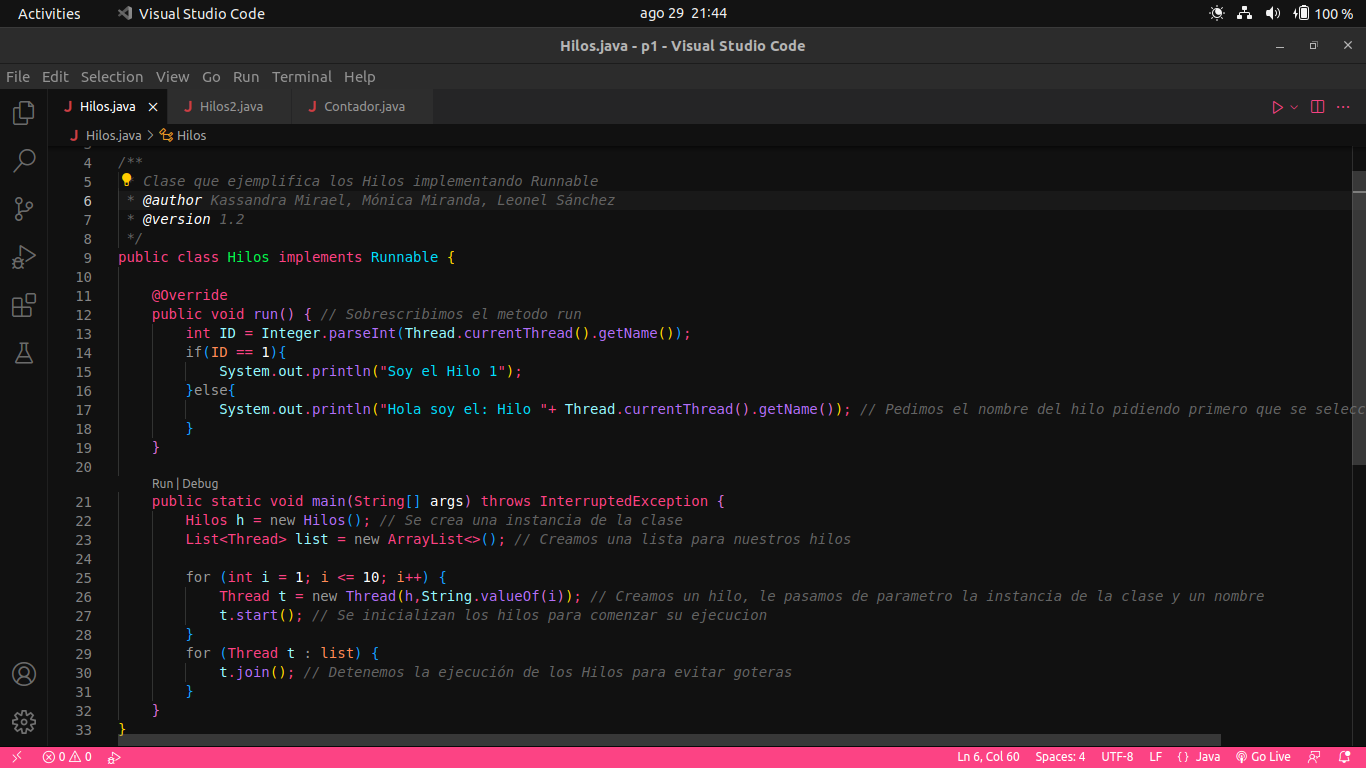
\includegraphics[scale=0.3]{p1_ej1.png}
    \caption{Código final: Introducción y jugando con Hilos}
    \label{fig:enter-label}
\end{figure}
\begin{enumerate}
    \item ¿Por qué se pone un \textit{InterruptedException} en el método \textit{main}?
    Porque los \textit{join()} pueden arrojar esta excepción si el hilo que está esperando es interrumpido por otro.
    
    \item ¿Para que sirve el método \textit{Join}?
    Pone una barrera a los hilos, que espera hasta que terminen los demás para continuar con su ejecución.
    
    \item ¿Qué pasa si no le hacemos \textit{Join} a los hilos?
    Puede haber goteras, ya que algunos hilos se pueden quedar olvidados, sin terminar, en algún proceso aunque el programa haya finalizado.
    
    \item Explica de manera consisa como usar Hilos extendiendo la clase \textit{Thread}.
    Definímos una nueva clase que hereda de \textit{Thread} y sobrescribimos el método \textit{run()} que se ejecutará en cada instancia o hilo cuando se inicien con el método \textit{start()}.
    
    \item ¿Cuáles son las ventajas en implementar \textit{Runnable} contra extender de \textit{Thread}? 
    Dado que en Java no tenemos extensión mutliple, a diferencia de extender sólo de la clase Thread, al implementar Runnable podremos implementar las interfaces que queramos, además de extender de alguna otra clase que necesitemos y reutilizan código fácilmente.
    
    \item ¿Se puede predecir el orden en el que se imprimira el mensaje de la clase \textit{Hilos}? 
    No, dependerá del calendarizador y del orden en que se ejecuten.
    
    \item En el archivo \textit{Hilos2.java}, ¿Qué pasa si sacamos la instancia de la clase \textit{“h”} de \textit{t1}, es decir, poner \textit{h} por ejemplo, antes de declar \textit{t1}?
    Permite que la instancia de la clase \textit{“h”} sea accesible dentro de Runnable.
    
    \item Explica como podriamos tener comportamientos diferentes implementando \textit{Runnable}.
    Podríamos obtener el identificador del hilo o los hilos que queramos diferenciar para capturarlos y aplicarles un comportamiento diferente.
% % % % % % % % % % % % % % % %
% % % % % % % % % % % % % % % %
% Preguntas de Matrices
% % % % % % % % % % % % % % % %
% % % % % % % % % % % % % % % %
    \item Para la sección 3 realiza lo siguiente:
    \begin{enumerate}
        \item Se incluyen una carpeta con 3 tipos de matrices, 10x10, 100x100 y 1000x1000, para cada prueba ejecutala y obtene el tiempo obtenido, tanto su versión secuencial asi como su versión concurrente, ¿Ves algun cambio significativo? ¿Mejoro el tiempo o empeoro? \\
        \textbf{R:} Mejora bastante, casi el doble, pero solamente en el caso de matriz de 1000 x 1000. En los casos pequeños el secuencial es mas rápido.
        \item Genera una gráfica con tus resultados obtenidos, usando 1,10 y 100 hilos.
        \begin{figure}[htbp]
            \centering
        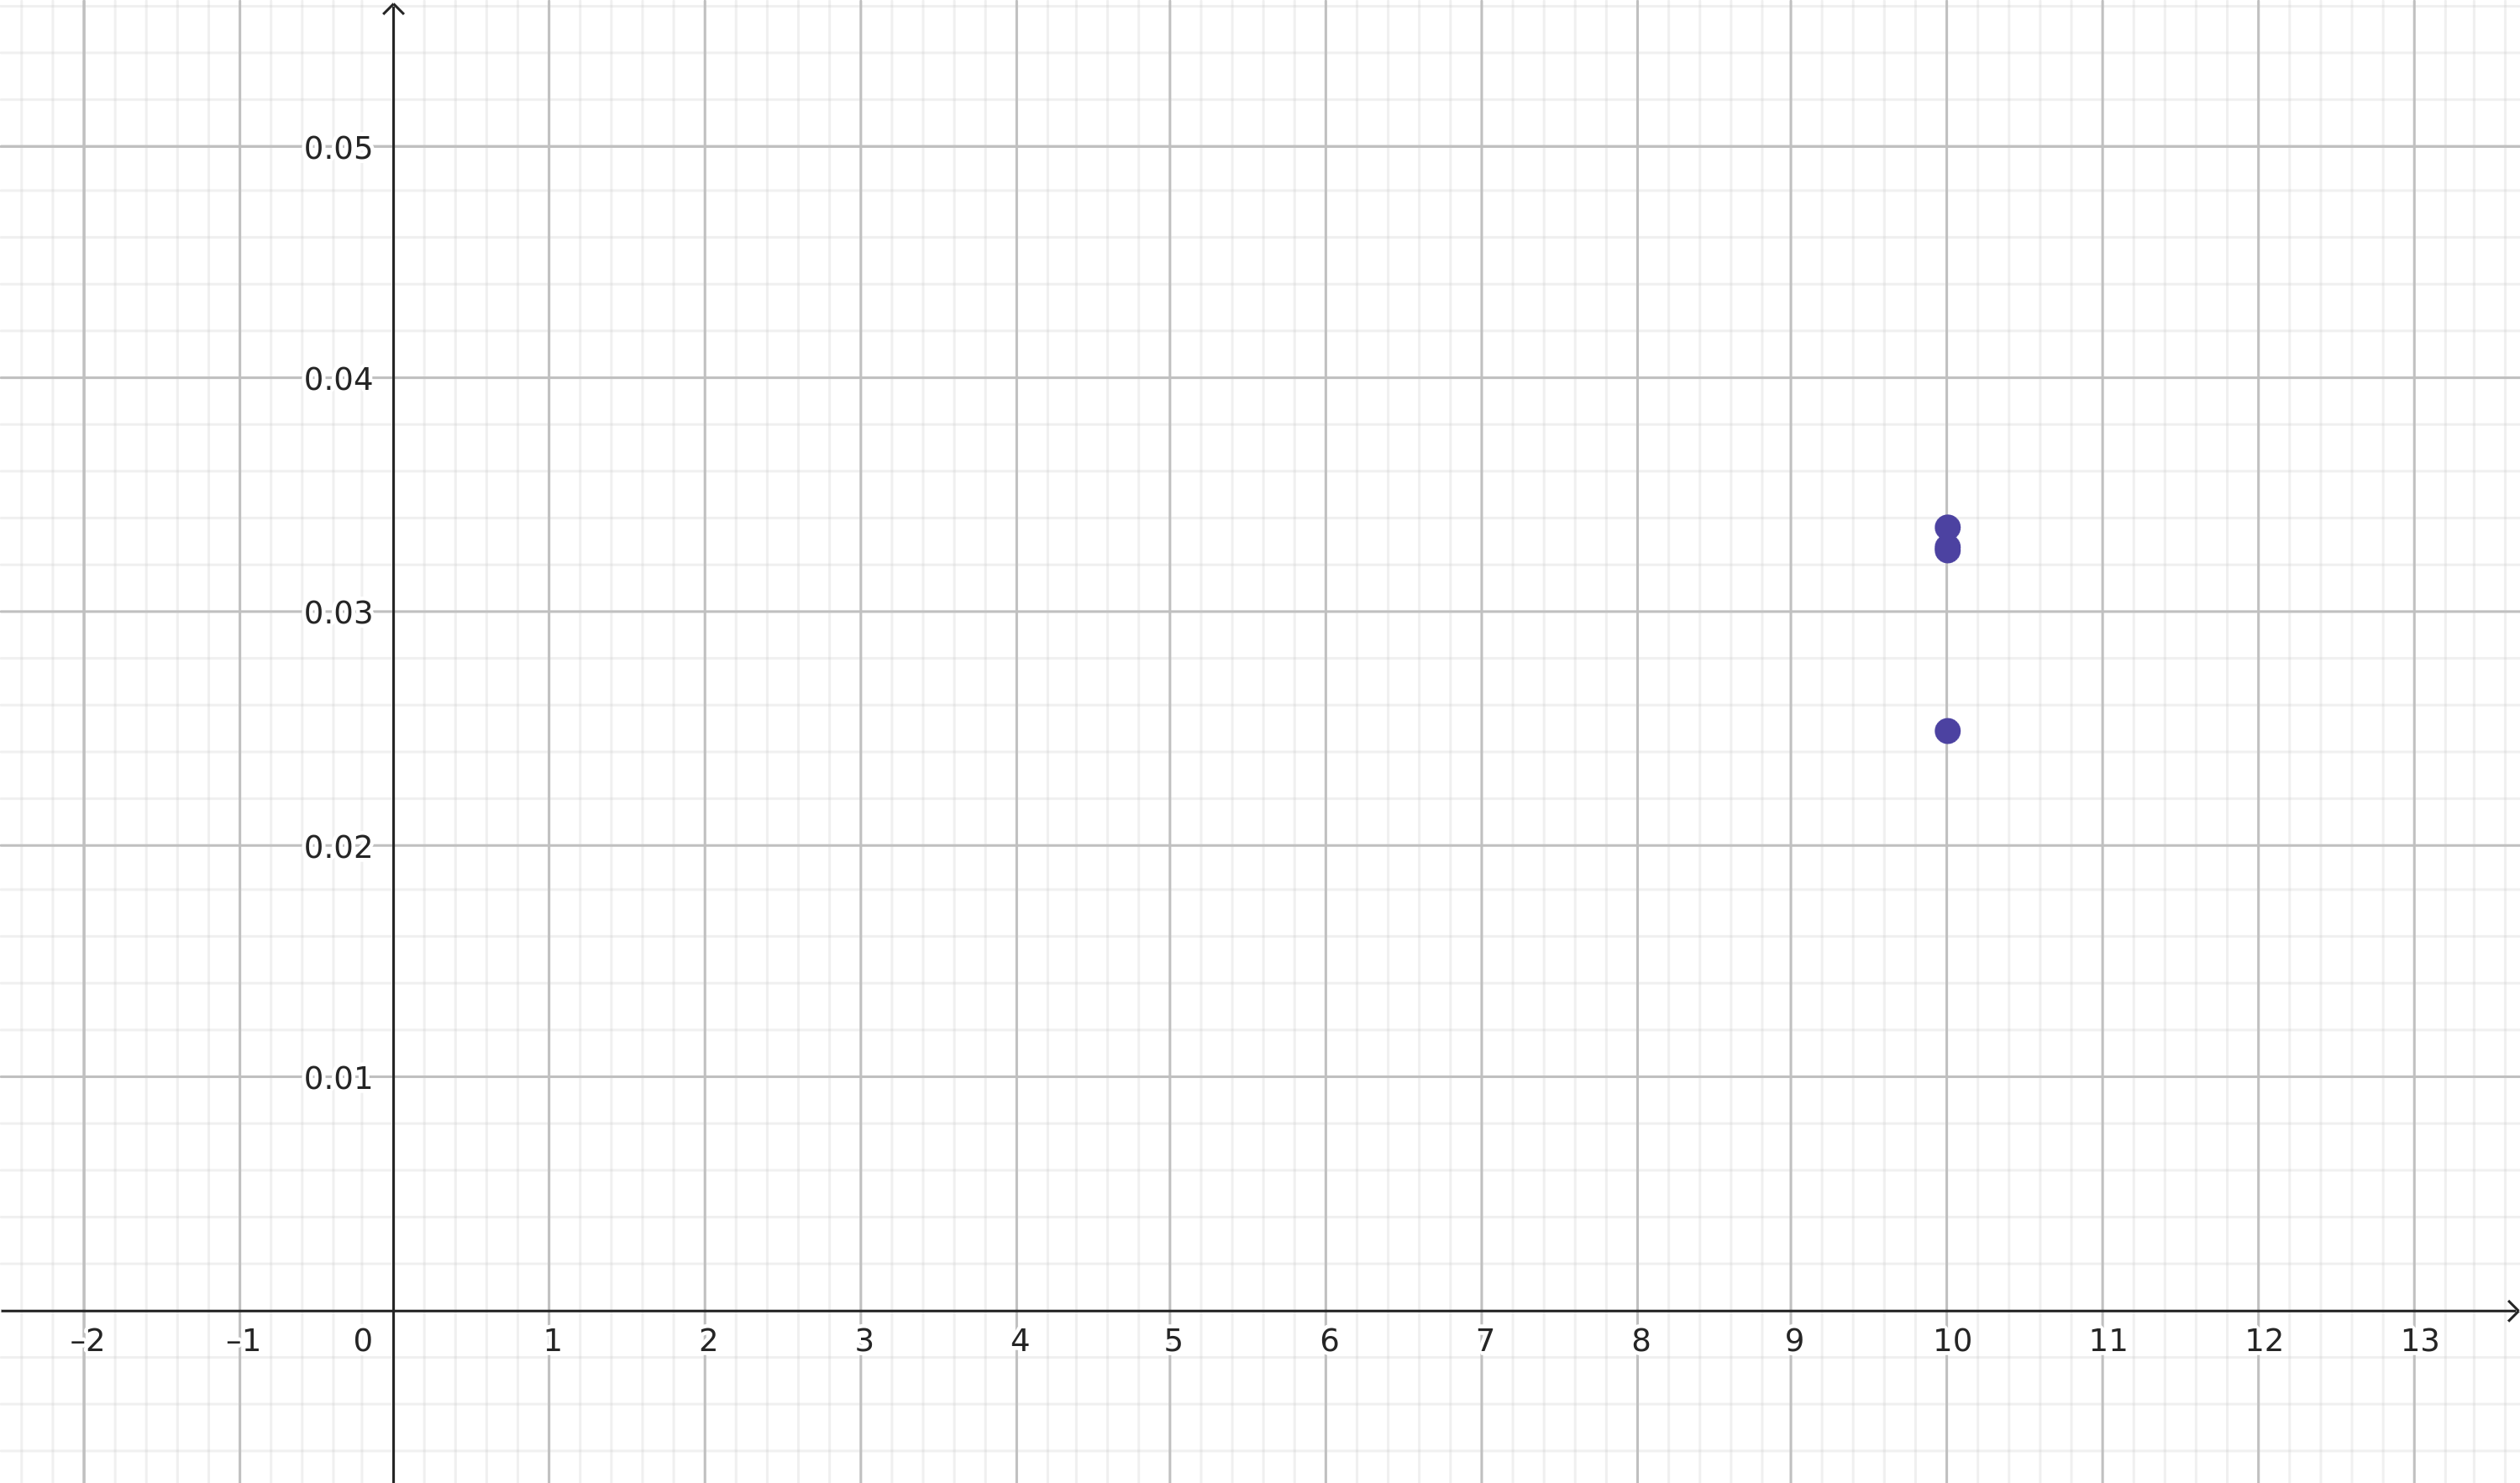
\includegraphics[scale=0.5]{images/M1.png}
        \caption{Resultados con la matriz de 10x10}
        \label{fig:enter-label} 
        \end{figure}
        \\\\
        \begin{figure}[htbp]
            \centering
        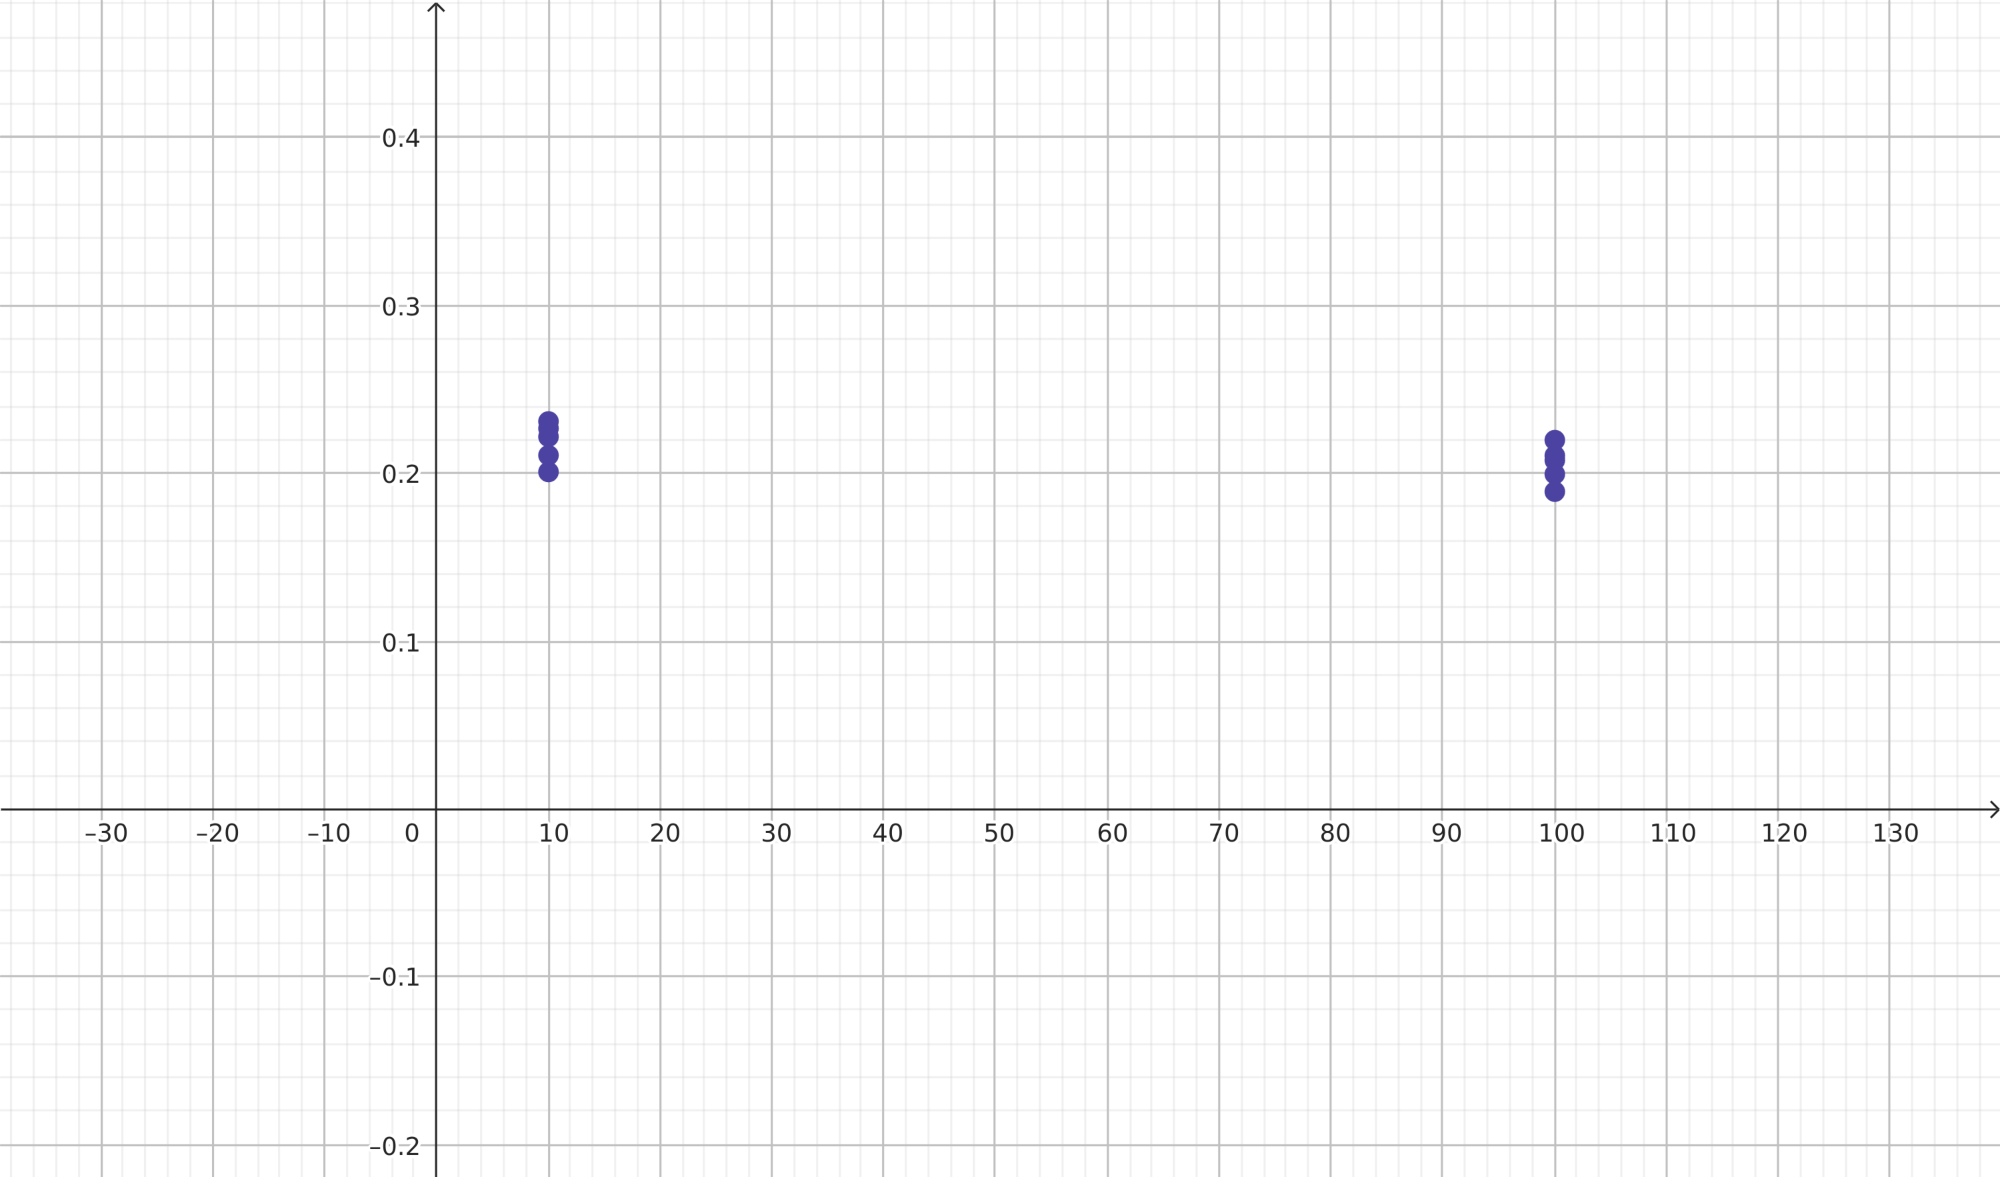
\includegraphics[scale=0.5]{images/M100.png}
        \caption{Resultados con la matriz de 100x100}
        \label{fig:enter-label} 
        \end{figure}
        \newpage
        \begin{figure}[htbp]
            \centering
        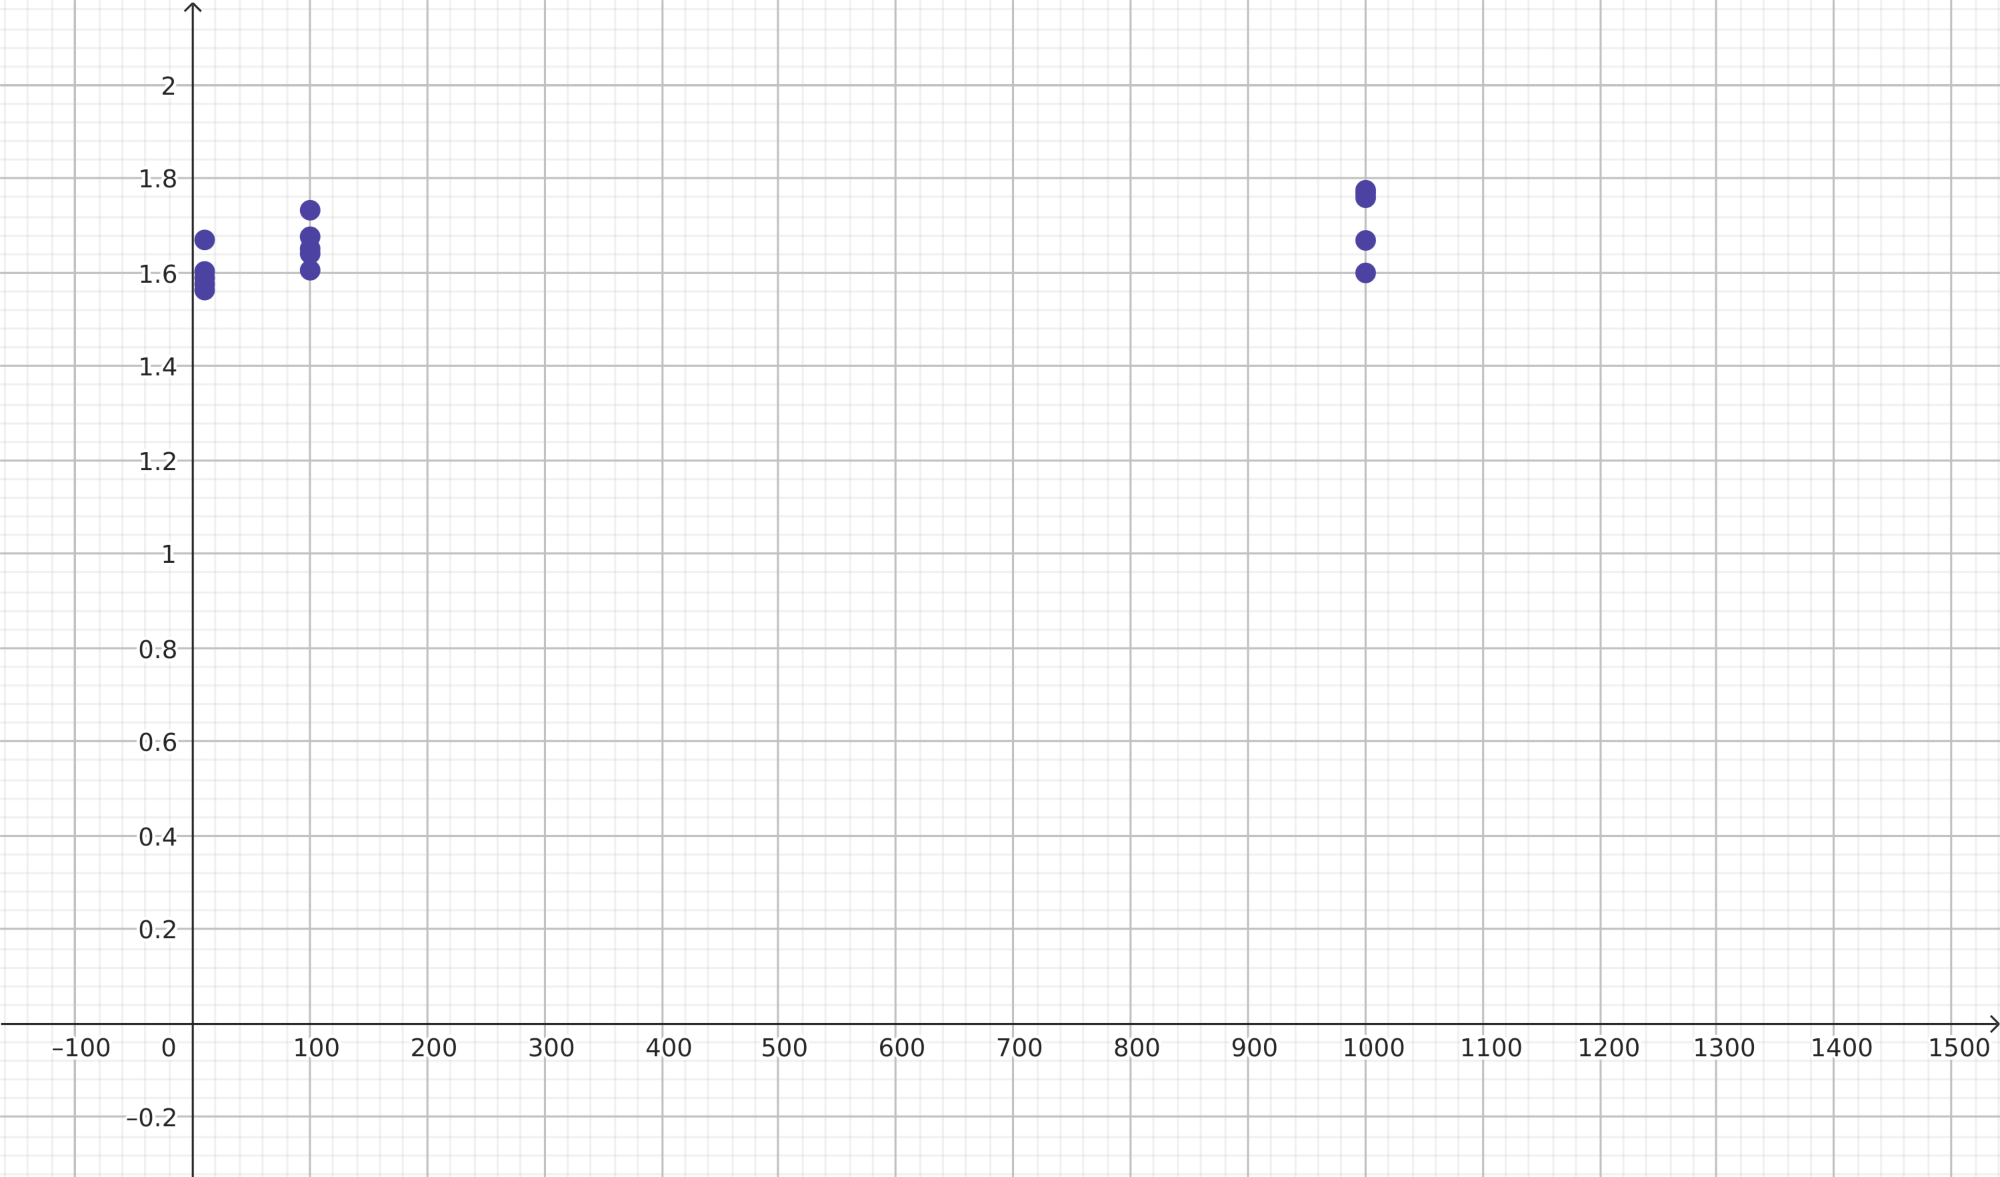
\includegraphics[scale=0.5]{images/M1000.png}
        \caption{Resultados con la matriz de 1000x1000}
        \label{fig:enter-label} 
        \end{figure}
        \textbf{Comentario:} como podemos observar en los casos con matrices pequeñas el concurrente es menos eficiente incluso que el secuencial, pero al trabajar con matrices mas grandes el secuencial es mucho mas efectivo.
        
        \item Finalmente pondremos a prueba la teoría , pues realizaremos la siguiente tabla con la info siguiente: 
        \begin{table}[h]
            \centering
            \begin{tabular}{ |c|c|c|c| }
                \hline
                 \# Hilos & Aceleración Teórica & Aceleración Obtenida & \% Código en paralelo \\       
                 \hline
                 10 en 10x10 & 1.1794 & 0.035 & 0.169 \\
                 \hline
                 10 en 100x100 & 1.1794 & - & 0.169 \\
                 \hline
                 10 en 1000x1000 & 1.1794 & - & 0.169 \\
                 \hline
                 100 en 10x10 & 1.2009 & 0.24 & 0.169 \\
                 \hline
                 100 en 100x100 & 1.2009 & 0.22 & 0.169 \\
                 \hline
                 100 en 1000x1000 & 1.2009 & - & 0.169 \\
                 \hline
                 1000 en 10x10 & 1.203 & 1.6 & 0.169 \\
                 \hline
                 1000 en 100x100 & 1.203 & 1.7 & 0.169 \\
                 \hline
                 1000 en 1000x1000 & 1.203 & 1.67 & 0.169 \\
                 \hline
            \end{tabular}            
        \end{table}                
        \item En la columna de Aceleración Teórica, utilizaremos la Ley de Amdahl y la compareremos con la Aceleración obtenida y responde la siguientes preguntas.
        \item ¿Se cumple siempre dicha ley?      
        \item ¿En que casos no se cumple?
        \item ¿Por qué crees que pasa esto? \\[2mm]
        \textbf{R (e,f,g):} Como comentamos antes, en las matrices de tamaño pequeño no cumple con esta ley, ya que al ser pequeños, hacer los hilos tarda mas que hacerlo en secuencial, con los tamaños grandes es incluso mejor que la aceleración teórico, nos imaginamos que con tamaños incluso mas grandes esta aceleración se acercaría al teórico. 
        \item ¿Cuál seria el nivel máximo de mejora?
        \textbf{R: } El nivel máximo suponemos que seria muy cercano al teórico, entre mas grande crezca la matriz mas se acerca a este.
        \newpage
        \item Para obtener una mejora aun mayor, en términos de Hardware, ¿Qué es mejor?, tener muchos mas núcleos con hilos o tener mayor frecuencia de reloj. Justifica. \\ 
        \textbf{R: } En general, depende que es lo que se necesita, si estamos el proceso que vamos a realizar tiene poco porcentaje de código en paralelo, nos conviene mas tener mayor frecuencia de reloj, y esto fácilmente lo podemos ver con la ley de ahmdal, acercando a P (el porcentaje en paralelo) a 1, y mayor numero de hilo, la aceleración es muchísimo.
        En este caso en particular nos conviene mayor frecuencia de reloj por lo antes mencionado.
        
    \end{enumerate}
    
    \item Responde TODAS las preguntas de la sección 4 de la parte practica (7 preguntas)
    \begin{enumerate}
        \item[1)] Ejecutar \textit{Contador.java} varias veces y ver que valores da, ¿Qué puedes decir de este resultado? El resultado varía.
        \item[2)] ¿Por qué lo da? Por las condiciones de carrera.
        \item[3)] Utiliza \textit{Thread.sleep} para dormir el hilo que selecciones, con el fin de realentizar al Hilo, ¿Por qué crees que hariamos esto? Para facilitar la observación de problemas.
        \item[4)] Finalmente, investiga para que funciona \textit{synchronized}. \\ Nos asegura que solo un hilo puede ejecutar ese método o bloque a la vez. Esto evita que varios hilos accedan y modifiquen datos compartidos, lo que podría llevar a resultados inconsistentes.
        \item[5)] Descomenta el bloque de codigo y ejecutalo. ¿Qué sucede cuando el bloque tiene \textit{synchronized}?. Tenemos menos variaciones en el resultado del contador. 
        \item[6)] Descomenta el siguiente bloque de codigo y ejecutalo nuevamente, ¿Qué diferencia ves? 
        El valor tiende a ser el mismo.
        \item[7)] ¿Por qué sucede esto? El \textit{''límite''} del lock. Ya que en el método, todos los subprocesos tendrán que esperar mientras el método lo ejecuta un subproceso. Mientras que en el bloque ``synchronized'', solo se aplicará al objeto entre paréntesis.
    \end{enumerate}
    \item Escribe lo aprendido con esta practica, asi como descubrimientos que obteniste mientras la realizaron.\\
En esta práctica, aprendimos sobre hilos, las condiciones de carrera que estos pueden tener y cómo pueden afectar los resultados de un programa. Logramos simular concurrencia e identificar problemas potenciales, y así hacer uso de \textit{synchronized} para evitarlos, logrando la sincronización segura de hilos. 
    
\end{enumerate}

\newpage
\section{Referencias}
[HS08] Maurice Herlihy and Nir Shavit. The Art of Multiprocessor Programming. Morgan Kaufmann Publishers Inc., San Francisco, CA, USA, 2008.\\[2mm]
Leyva Castillo, L. A. (2023). Parte 1 [Archivo de video]. Ayudantía Lab (24/08/23). Google Drive. URL:
\url{ https://drive.google.com/file/d/1Dd__2dJyiHN6C1Op1qAFA-Uu2MPGeImg/view?usp=drive_link } (Consultado el: 29 Agosto 2023).  \\[2mm]
Synchronized methods. Synchronized Methods (The JavaTM Tutorials \& Essential Java Classes \& Concurrency). Disponible en: \url{ https://docs.oracle.com/javase/tutorial/essential/concurrency/syncmeth.html } (Consultado el: 30 Agosto 2023). \\[2mm]
Intrinsic locks and synchronization. Intrinsic Locks and Synchronization (The JavaTM Tutorials \& Essential Java Classes \& Concurrency). Disponible en: 
\url{ https://docs.oracle.com/javase/tutorial/essential/concurrency/locksync.html } (Consultado el: 31 August 2023). 
\end{document}
